\documentclass[11pt]{article}
\usepackage[utf8]{inputenc}
\usepackage{subcaption}
\usepackage{amsmath}
\usepackage{amssymb}
\usepackage{hyperref}
\usepackage{titlesec}
\usepackage{fancyhdr}
\usepackage{graphicx}
\usepackage{tcolorbox}
\usepackage{multirow}
\usepackage[rightcaption]{sidecap}
\usepackage{verbatim}
\usepackage[backend=bibtex]{biblatex}
\usepackage{blindtext}
\usepackage{multicol}
\usepackage{algorithm}
\usepackage{algpseudocode}
\usepackage [ a4paper , hmargin =1 in , bottom =0.8 in ] { geometry }
\hypersetup{
    colorlinks=true,
    linkcolor=blue,
    filecolor=magenta,      
    urlcolor=cyan,
}
\usepackage{xcolor}
\newcommand\ytl[2]{
\parbox[b]{10em}{\hfill{\color{cyan}\bfseries\sffamily #1}~$\cdots\cdots$~}\makebox[0pt][c]{$\bullet$}\vrule\quad \parbox[c]{8cm}{\vspace{7pt}\color{red!40!black!80}\raggedright\sffamily #2\\[7pt]}\\[-3pt]}
\usepackage{titling}

\setlength{\droptitle}{-7em} 

\bibliography{bibliography}
% Add header and footer code here
\fancyhead[L]{CS349}
\fancyhead[C]{XData Extensions}
\fancyhead[R]{Project Report}
\fancyfoot[C]{Page \thepage}

\DeclareMathOperator*{\maxi}{max}
\DeclareMathOperator*{\mini}{min}

\setlength{\parindent}{0pt}

\graphicspath{{images/}}

\begin{document}


\title{CS349: Course Project \\ \vspace{0.5em} \Huge \textbf{XData Extensions} \\ \vspace{0.5em} \Large Project Report}
\date{Spring 2025} % Use today's date or remove for no date
\author{Satyankar Chandra (22B0967) \and Ayan Tanwar (22B0931) \and Harsh Kumar (22B0973) \and Gourish Garg (22B0915)} % Use \and for multiple authors

\maketitle
\thispagestyle{empty} % Remove header/footer from title page

\tableofcontents

\vfill

\begin{center}
    \Large \textbf{Source Code:} \href{https://github.com/SuperSat001/CS349-Course-Project/tree/main}{https://github.com/SuperSat001/CS349-Course-Project/}
\end{center}

\begin{center}
    \Large \textbf{Guide: Prof. S. Sudarshan and Prof. Suraj Shetiya} \\
    Dept. of Computer Science and Engineering, IIT Bombay
\end{center}
\clearpage
\pagestyle{fancy}

\newpage

\section{Introduction}

This report documents the work done in the CS349 course project during the Spring 2024 - 2025 semester. Our project topic is \textbf{XData Extensions}, where we aim to extend the functionality of the XData system. 

\medskip

During this project, our team has implemented several features and improvements to the existing XData platform. The goal of this project is to enhance the usability and functionality of the XData system, making it more user-friendly for both students and faculty members.

\medskip

For demonstration purposes, we have created a simple web application that showcases the new features our team has developed in isolation. This application serves as a minimal working example of our work, and code for the same is available in the GitHub repository linked above. We have also ensured that our features are compatible with the existing XData system. At our backend, we have used the same database schema as XData to store data about students, courses, and assignments.

\medskip

Our team has spent a considerable amount of time and effort on this project throughout the semester. The rough timeline of our work is as follows:

\begin{itemize}
    \item \textbf{Week 1-2:} Setting up the project, \textbf{creating a small web application which uses PGLite} to host a local in-browser database. Deciding on the features to be implemented.
    \item \textbf{Week 3-5:} Implementing features for \textbf{Query Planning, Syntax Constrained Querying and Multi-database setup} in PGLite. Improving the ReactJS frontend to provide a better user experience for these features.
    \item \textbf{Week 6-7:} Integrating the \textbf{current XData schema} to store assignments and evaluated data. Implementing UI for instructors to create courses and assignments, and for students to attempt them. Implementing a \textbf{Query Playground} for students to test their queries and get feedback. 
    \item \textbf{Week 8:} Implementing other QoL improvements such as \textbf{Query History}, a simple \textbf{version control system} for loaded databases, enhancing \textbf{Import/Export} functionality, and other minor features.
    \item \textbf{Week 9:} Finalizing the project, UI improvements, basic security testing and bug fixing.
\end{itemize}

Around Week 6, we also submitted a mid-semester report and part of the code to the instructors. We also met with them to discuss our progress and get crucial feedback on our work. The feedback was very helpful in guiding us towards the final implementation - especially with the XData integration (using the same database schema) as well as some of our core features. Based on the feedback, we discarded some of our initial ideas and focused on the features that would be most useful for students and instructors and are easier to integrate with the existing XData system.

\medskip

Full details of the features we have implemented are discussed in section \ref{sec:contributions}. We have also included in section \ref{sec:future-work} a list of improvements and features that we would like to implement given more time in the future.

\newpage

\section{Project Goals}

The main problem statement we started with was as follows:

\begin{tcolorbox}[colframe=blue, colback=white, title=XData Extensions Problem Statement]
Extend XData to support in-browse postgresql execution using \href{https://pglite.dev/}{https://pglite.dev}.  Make sure everything runs from local resources so it can be run for exams without external internet.  This allow each user to run in their own database without accessing any central database.  The next step is to extend XData system to run the queries in browser rather than on a backend database. 
\end{tcolorbox}

With this in mind, our team started brainstorming ideas for features to implement. We tried to code the features in isolation, and then integrate them into a single web application. This helped us to work on the features independently and in parallel, while also ensuring that they would work together in the final product.

\medskip

We started with the following features as a part of our initial project proposal:
\begin{itemize}
    \item Evaluation Plans and Query Optimization
    \item Query Profiling and Runtime Analysis
    \item Support for Concurrent Queries and Multiple Databases
    \item Adding Syntactic Constraints to Queries
    \item Improvements to the XData UI to better support the new features
\end{itemize}

After discussing with the instructors, we received positive feedback on our implementation of the Query Planning features and frontend UI. However, it was evident that some of our initial ideas (on Query Profiling) were not feasible within the scope of the project and it would be better to focus on the remaining features along with the their integration with the current XData system. After getting access to the XData GitLab and the database schema, we spent most of our time during the second half on the integration aspect of the project.

\medskip

The final set of implemented features is presented in the next section. 

\section{Main Contributions}
\label{sec:contributions}
In this section, we will discuss the main features we have implemented in our project. These features are roughly listed in the order of typical user interaction. We also have a few other features which are not directly related to user interaction, but are important for the overall functionality of the system.

\subsection{User Experience Features}
\subsubsection{Course Creation or Selection \ref{fig:add_course}}
We allow instructors to modify assignments/schema of existing courses or create new courses. Changes to a course are automatically reflected in the database with the XData schema.

\begin{figure}[h!]
    \centering
    \begin{subfigure}[b]{0.3\textwidth}
        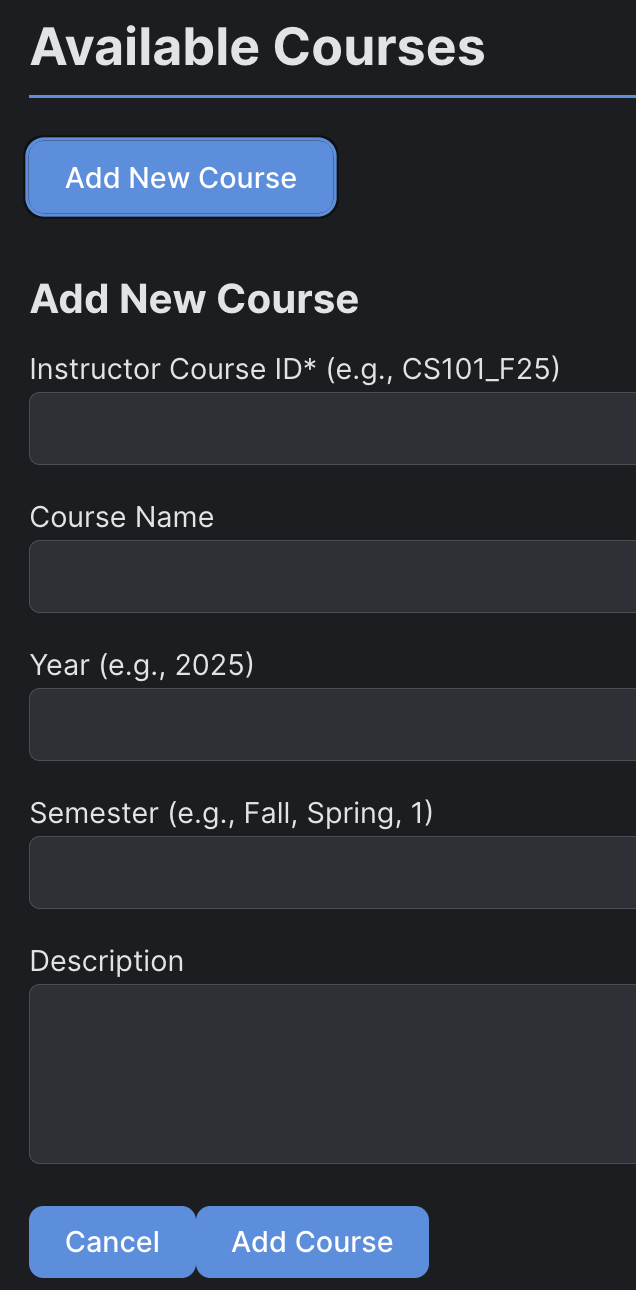
\includegraphics[width=\textwidth]{add_course.png}
        \caption{Adding a Course}
        \label{fig:add_course}
    \end{subfigure}
    \hfill
    \begin{subfigure}[b]{0.55\textwidth}
        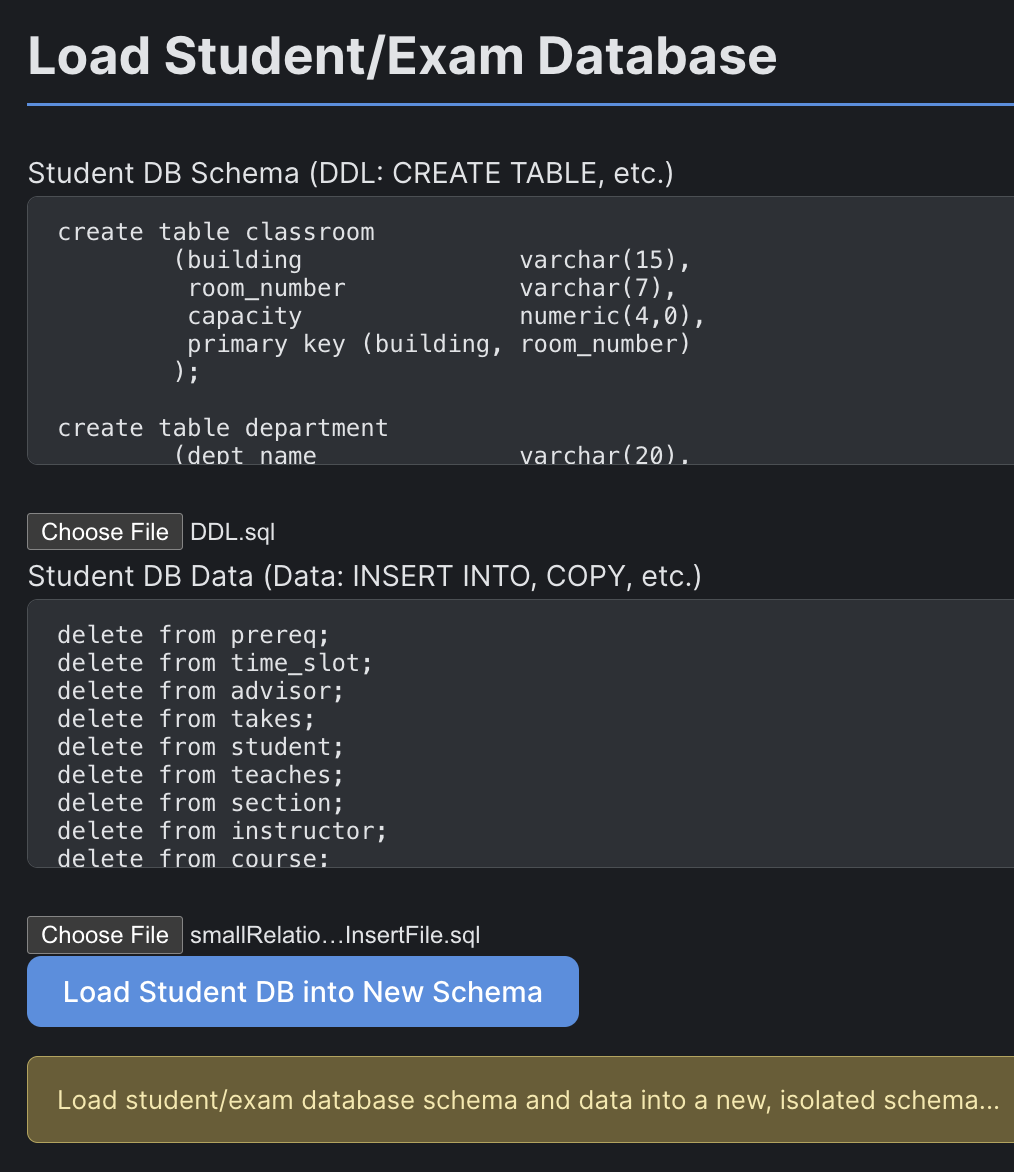
\includegraphics[width=\textwidth]{load_db.png}
        \caption{Loading a Database}
        \label{fig:load_db}
    \end{subfigure}
\end{figure}

\subsubsection{Loading and Modifying Databases \ref{fig:load_db}}
Both instructors and students can load databases from local files or by manually entering the schema. The databases are stored in the browser's local storage via PGLite. The databases are fully isolated from each other, and users can switch between them anytime without any issues. Tuples can be added, modified or deleted from the database at any time.

\subsubsection{Assignment Creation and Deployment \ref{fig:assn}, \ref{fig:assn_qn}}
After selecting a course and loading the database schema, instructors can create assignments for students. The assignments are again stored in the XData schema, and can be modified or deleted at any time. Instructors can supply a valid SQL query for each question in the assignment, which will be used to evaluate the students' submissions. Students can then attempt the assignments using the Query Playground.

\begin{figure}[h!]
    \centering
    \begin{subfigure}[b]{0.45\textwidth}
        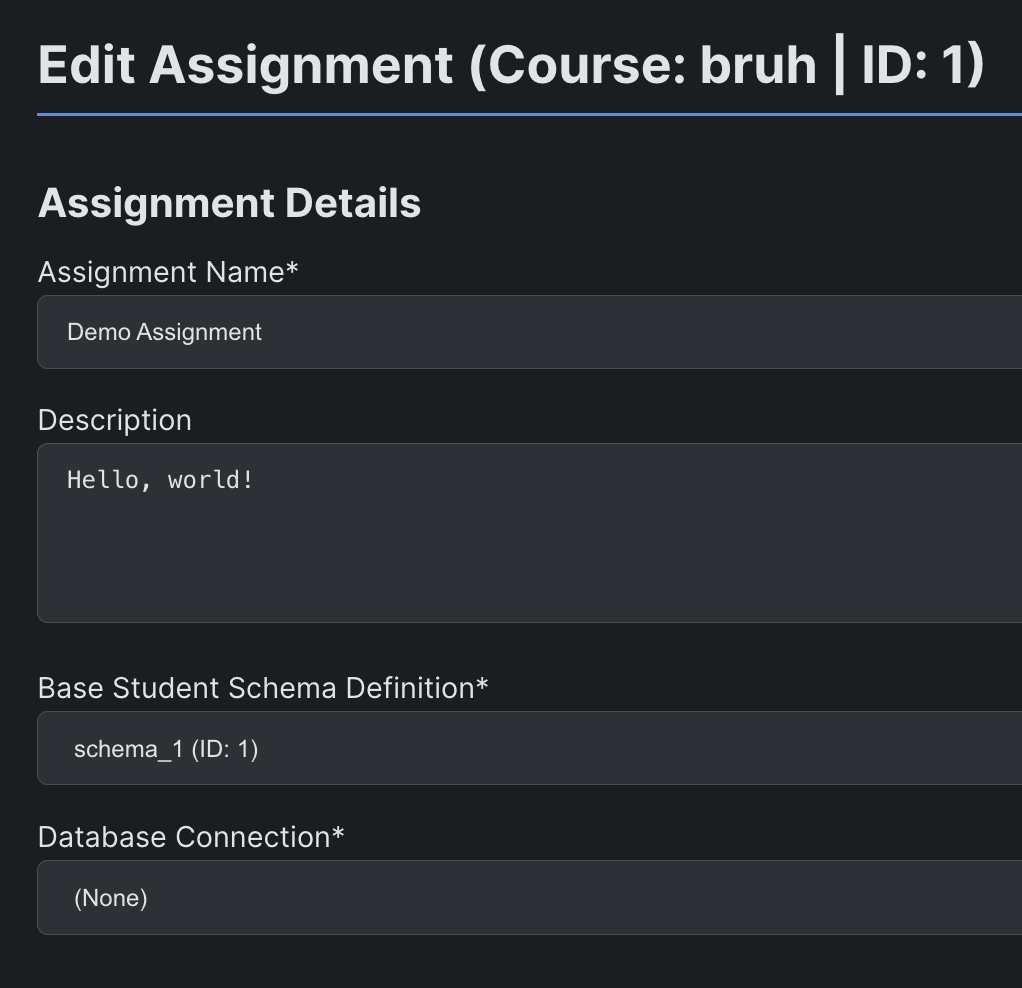
\includegraphics[width=\textwidth]{assn.png}
        \caption{Editing an Assignment}
        \label{fig:assn}
    \end{subfigure}
    \hfill
    \begin{subfigure}[b]{0.35\textwidth}
        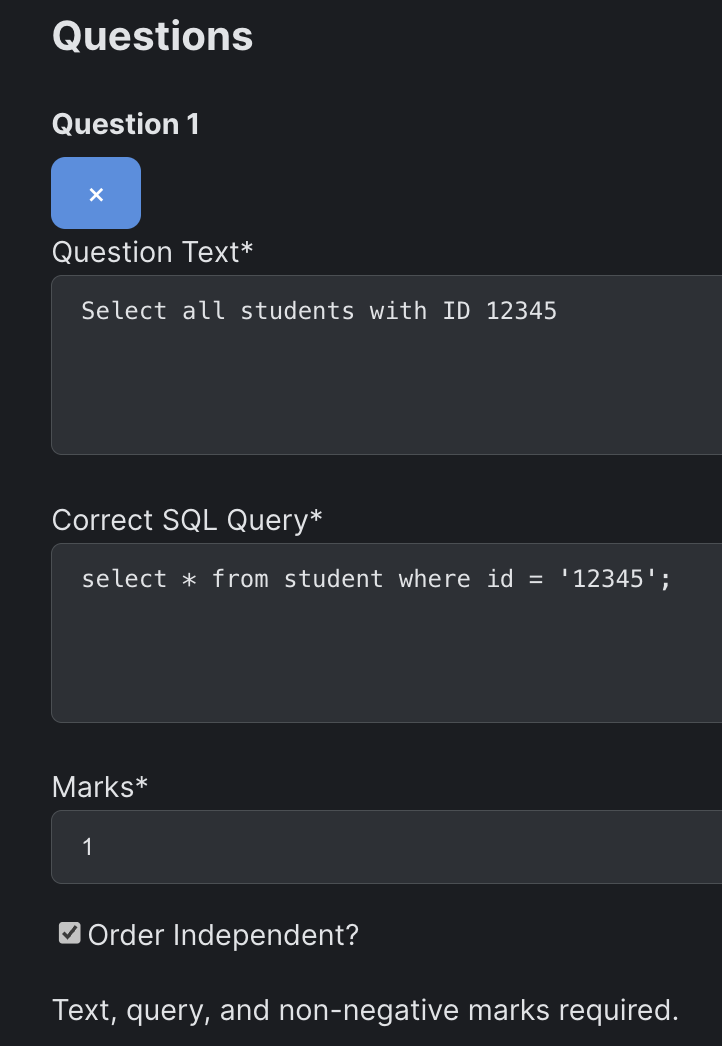
\includegraphics[width=\textwidth]{assn_qn.png}
        \caption{Making a Question}
        \label{fig:assn_qn}
    \end{subfigure}
\end{figure}

\subsubsection{Query Playground \ref{fig:play_r}, \ref{fig:play_w}}
The Query Playground is a convenient interface for students to test their queries and get instant feedback. The playground allows students to run any SQL query on the loaded database, and provides a simple interface to view the results. Students can load their own data with the same schema, and compare the results with the expected output. 

\begin{figure}[h!]
    \centering
    \begin{subfigure}[b]{0.4\textwidth}
        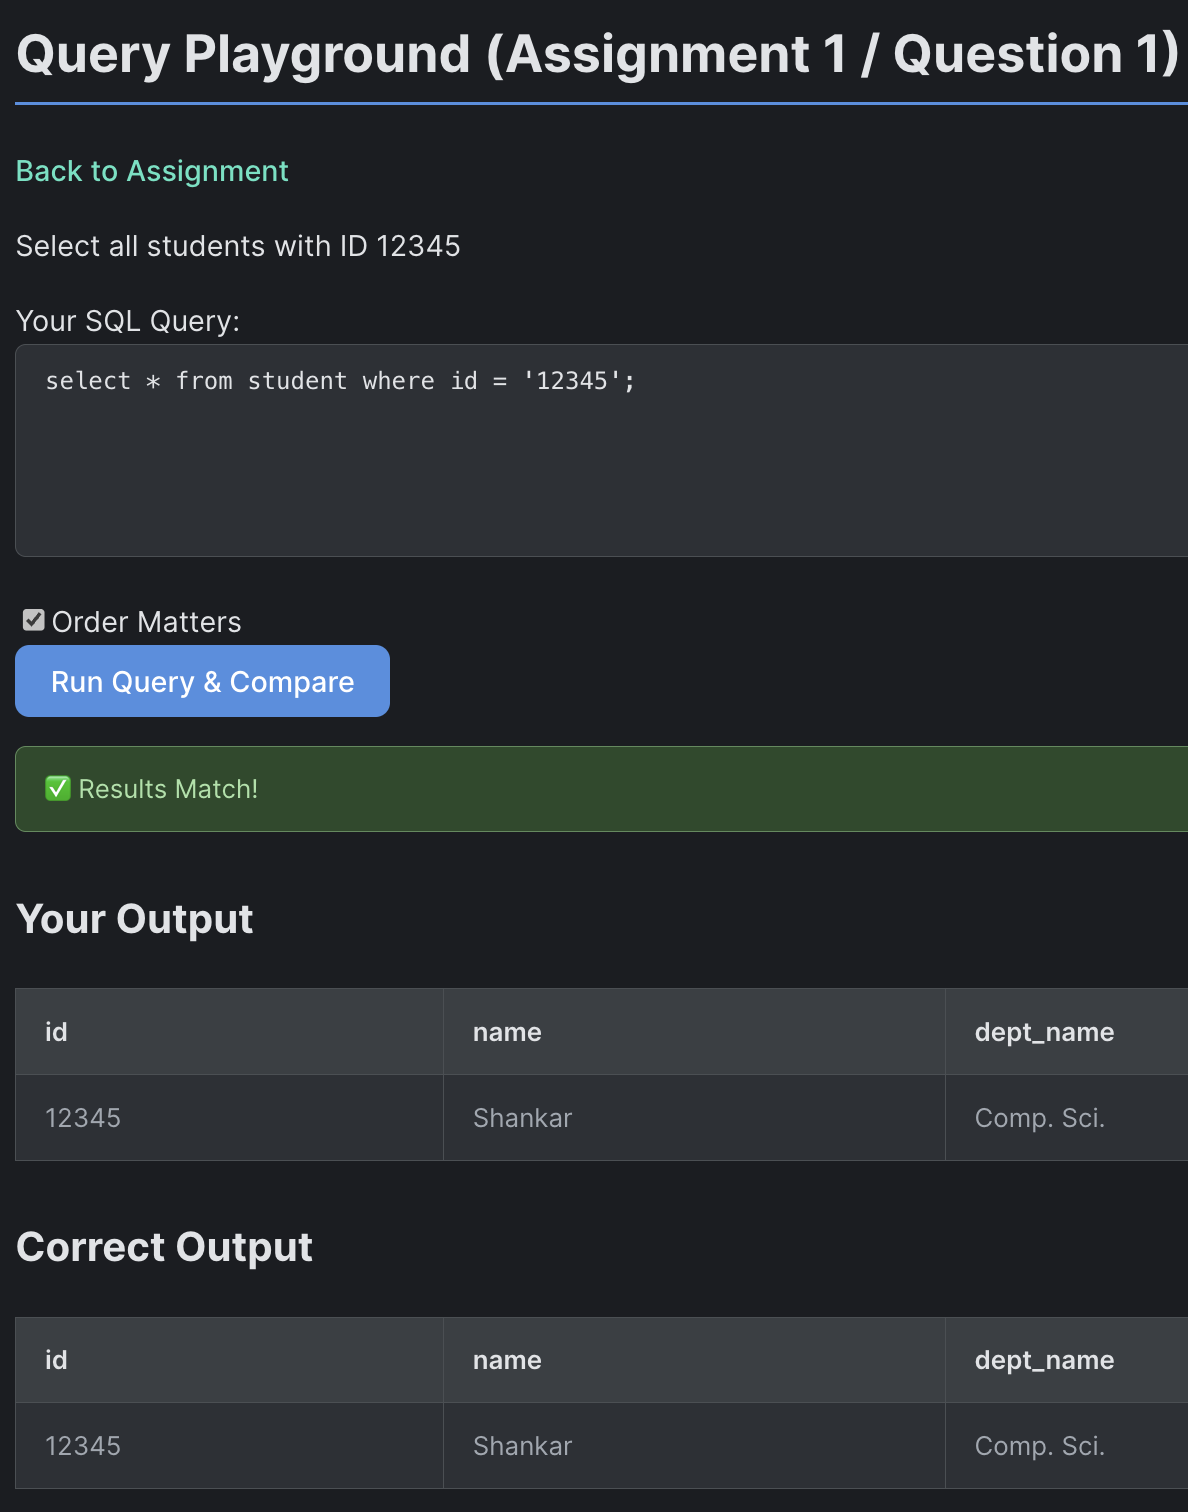
\includegraphics[width=\textwidth]{play_right.png}
        \caption{Right Answer}
        \label{fig:play_r}
    \end{subfigure}
    \hfill
    \begin{subfigure}[b]{0.45\textwidth}
        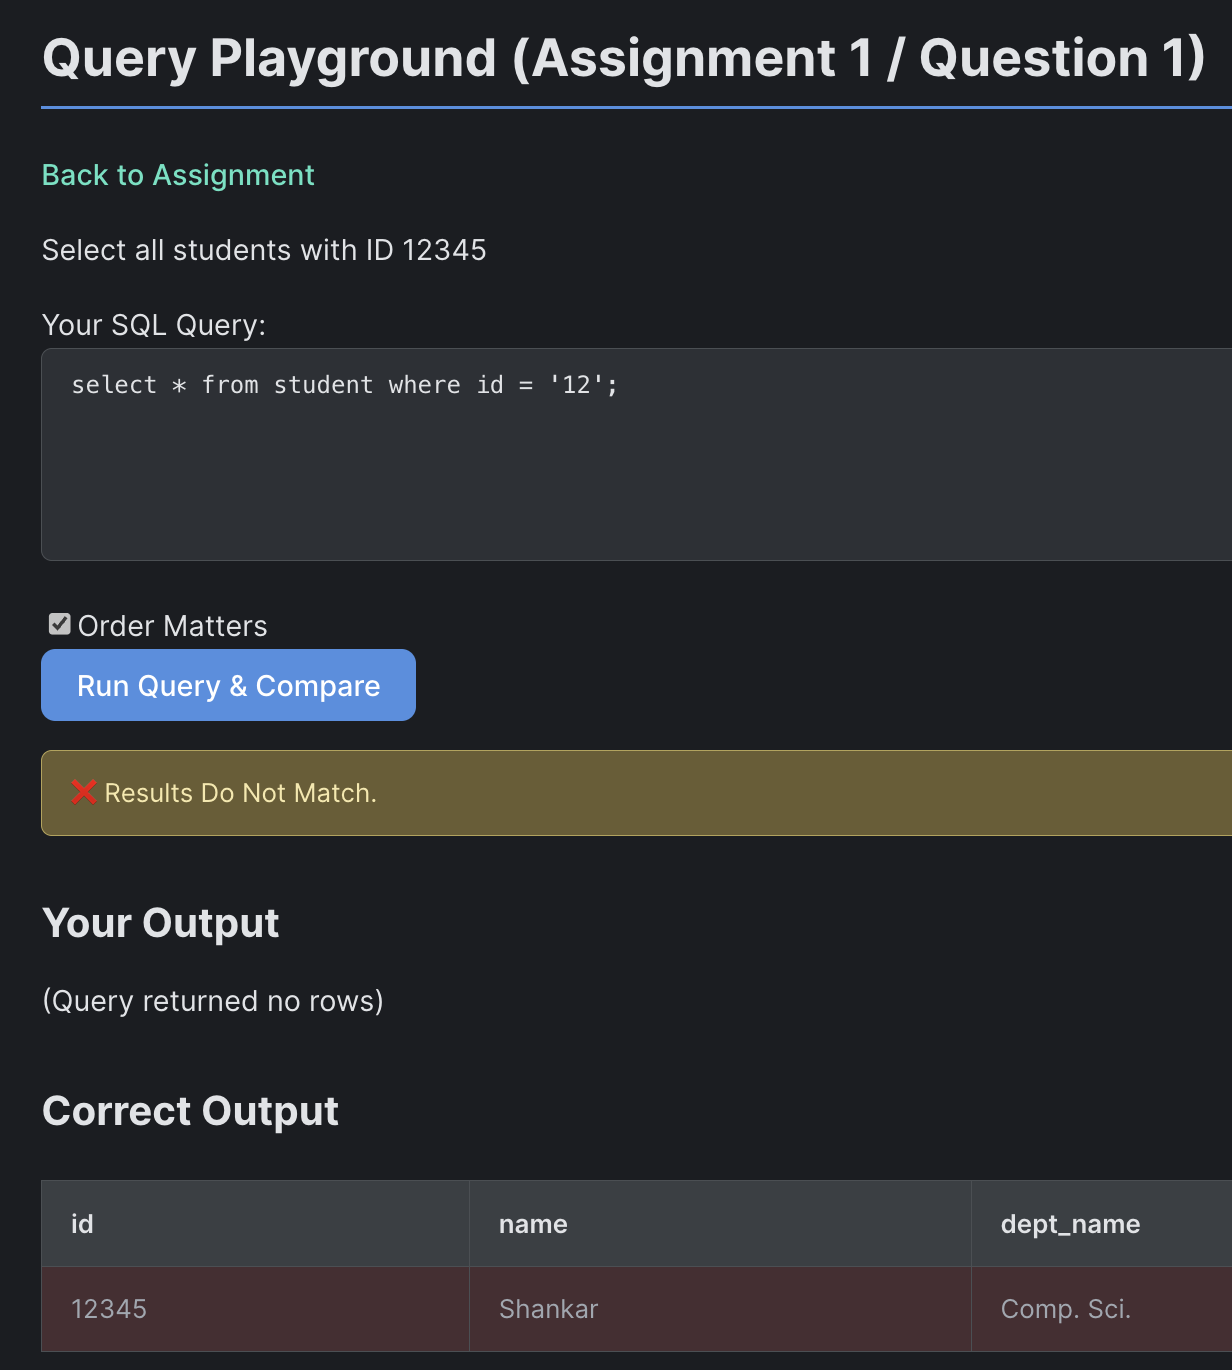
\includegraphics[width=\textwidth]{play_wrong.png}
        \caption{Wrong Answer}
        \label{fig:play_w}
    \end{subfigure}
\end{figure}

\subsubsection{Query Planner \ref{fig:seq_plan}, \ref{fig:index_plan}}
PostgreSQL typically uses a cost-based query planner to determine the best execution plan for a given query. However, it does not allow users to specify their own query plans. We have implemented this functionality by setting and unsetting particular flags so that query is forced to run in a particular way. This allows users to experiment with different query plans and see how they affect the performance of the query.

\begin{figure}[h!]
    \centering
    \begin{subfigure}[b]{\textwidth}
        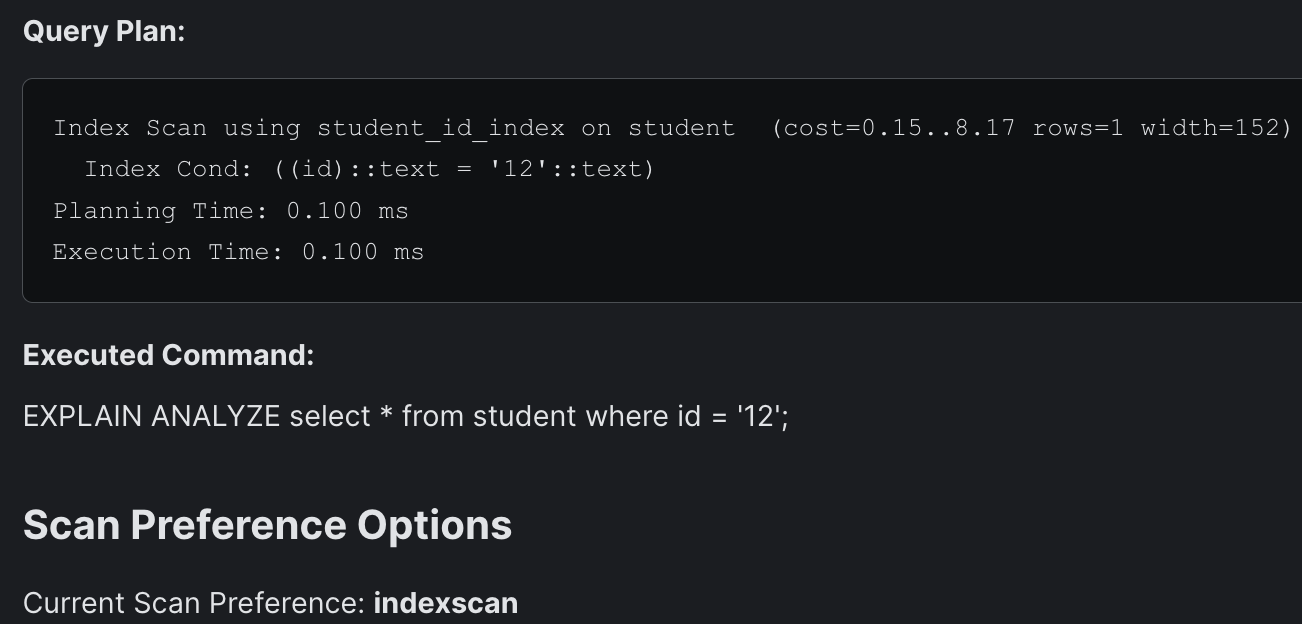
\includegraphics[width=\textwidth]{index_plan.png}
        \caption{Forcing Index Scan}
        \label{fig:index_plan}
    \end{subfigure}
    \hfill
    \begin{subfigure}[b]{\textwidth}
        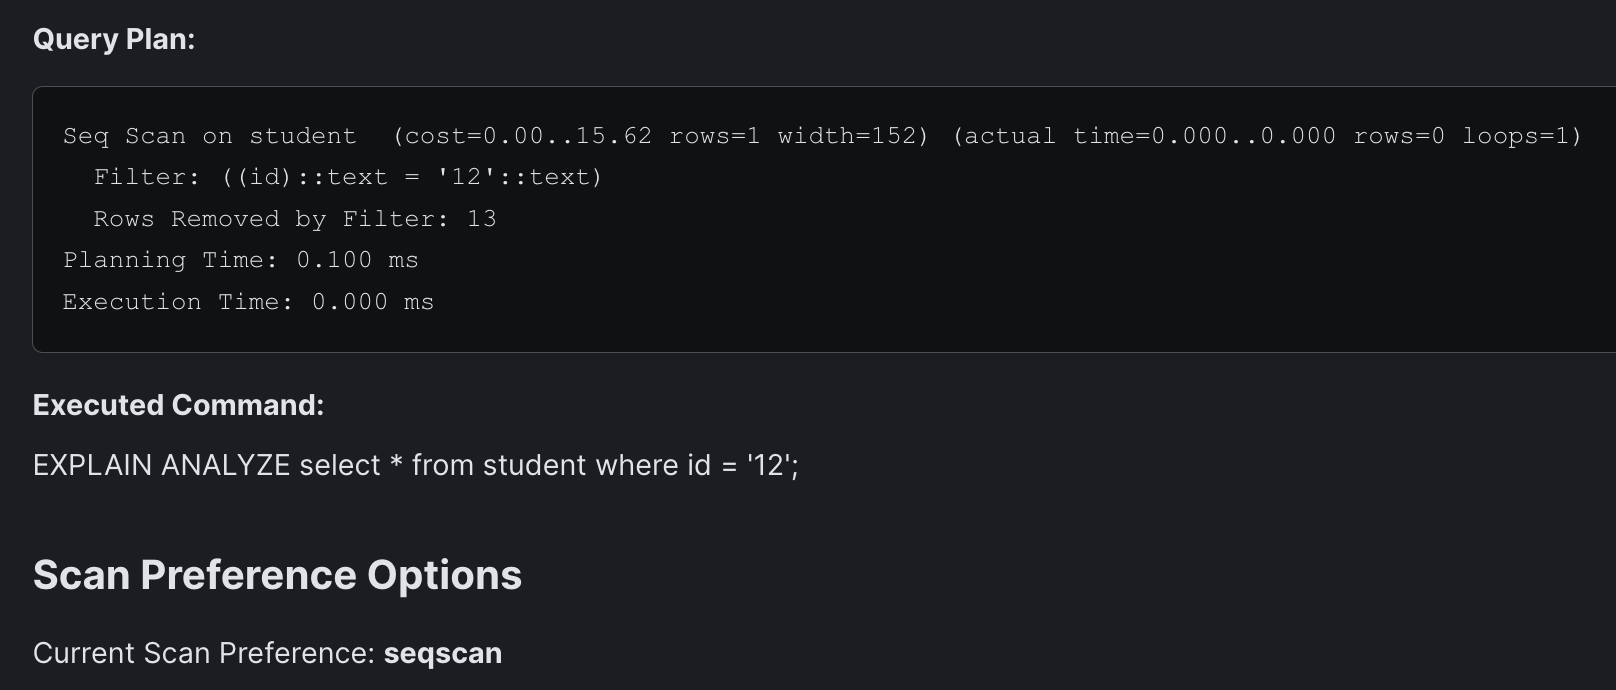
\includegraphics[width=\textwidth]{seq_plan.png}
        \caption{Forcing Sequential Scan}
        \label{fig:seq_plan}
    \end{subfigure}
\end{figure}

\subsubsection{Syntactic Constraints on Queries}
Often, instructors want to enforce certain syntactic constraints on the queries submitted by students. For example, they may want to ensure that students do not use certain keywords or functions in their queries. We tried to implement this feature by using a simple parser on the query string and whitelisting/blacklisting certain keywords. However, this approach becomes overly restrictive for complex constrains and hence this feature is still a work in progress.

\subsection{Utility Features}

\subsubsection{Database Viewer \ref{fig:db_view}}
We have implemented a simple database viewer which allows users to view and edit the contents of the database. The viewer displays the tables in the database, along with their schema and data. Users can also add, modify or delete tuples from the database using this interface. This feature is useful for users who want to quickly view the contents of the database without having to run any queries.
\begin{figure}[h!]
    \centering
    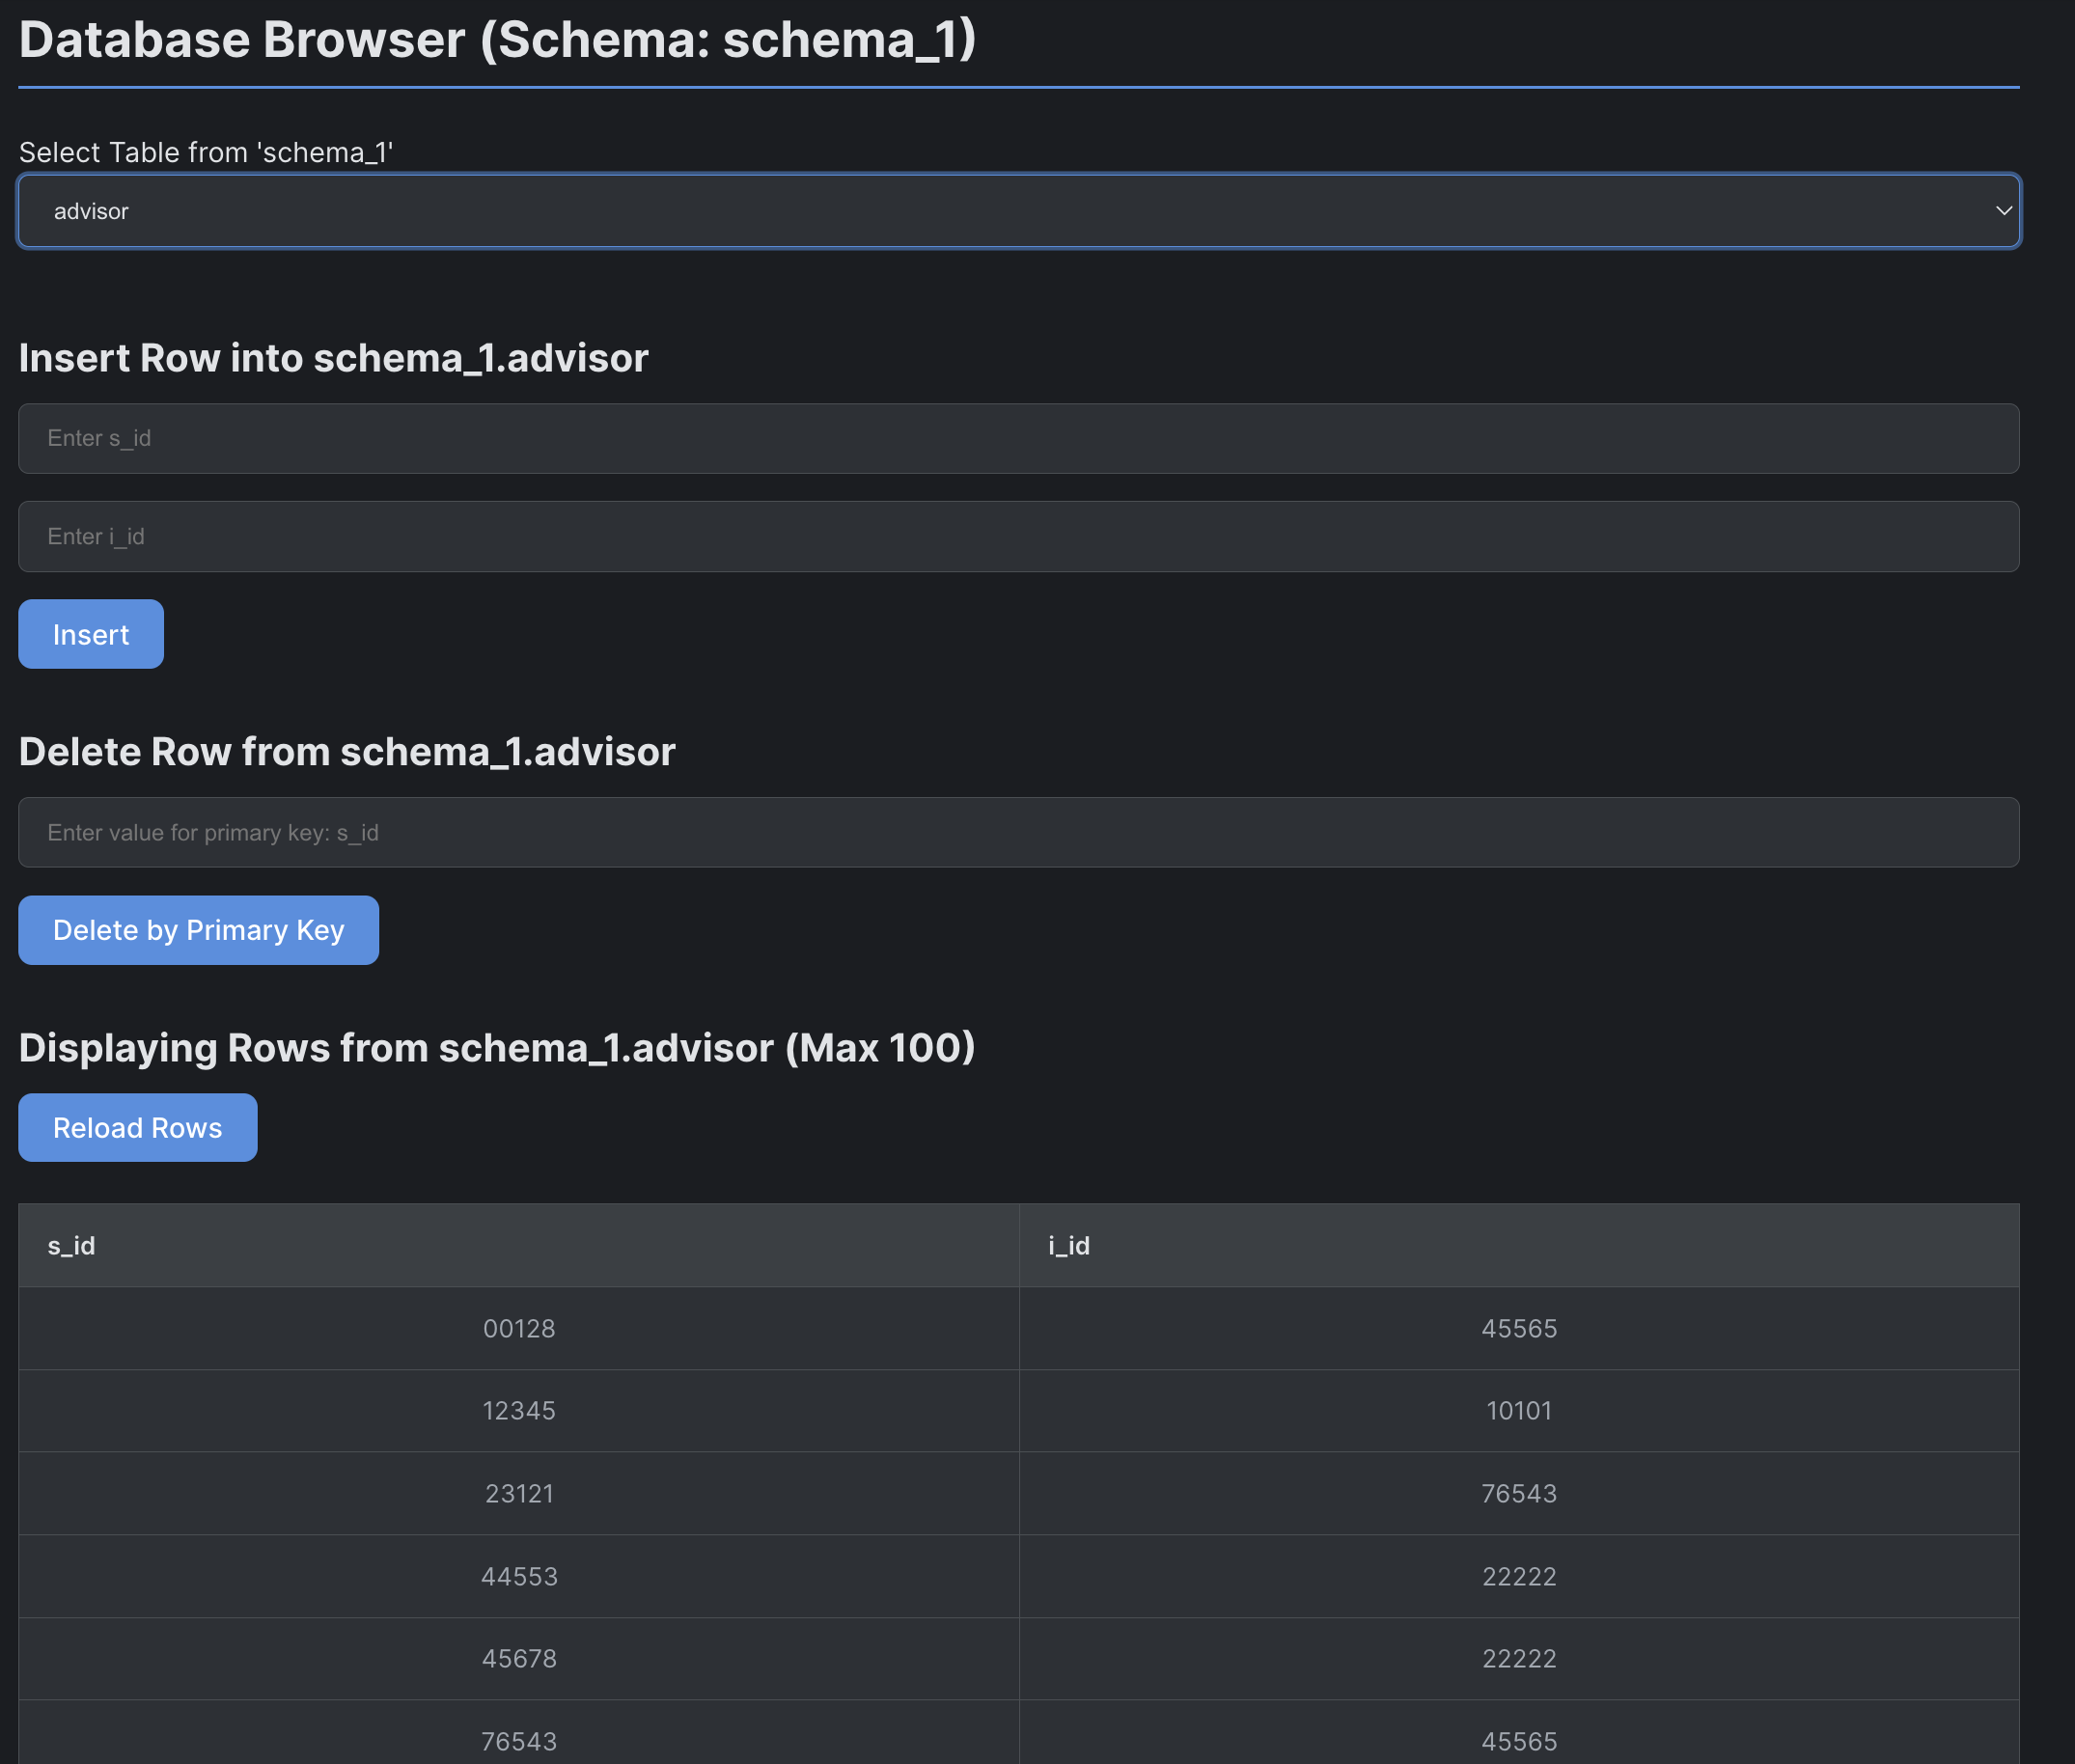
\includegraphics[width=0.8\textwidth]{browse.png}
    \caption{Database Viewer}
    \label{fig:db_view}
\end{figure}

\subsubsection{Query History Tracker \ref{fig:history}}
We have implemented a simple query history tracker which displays the last 10 queries run by the user in a side panel. There is a button to copy the query to the clipboard, so that the user can easily reuse it. This feature is useful for users who want to quickly access their previous queries without having to retype them.

\begin{figure}[h!]
    \centering
    \begin{subfigure}[b]{0.45\textwidth}
        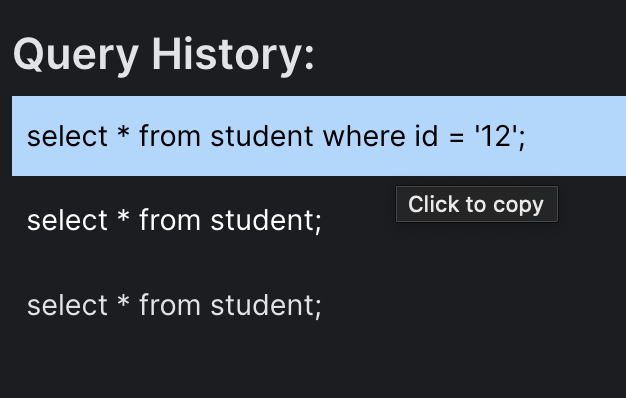
\includegraphics[width=\textwidth]{history.png}
        \caption{Showing Query History}
        \label{fig:history}
    \end{subfigure}
    \hfill
    \begin{subfigure}[b]{0.45\textwidth}
        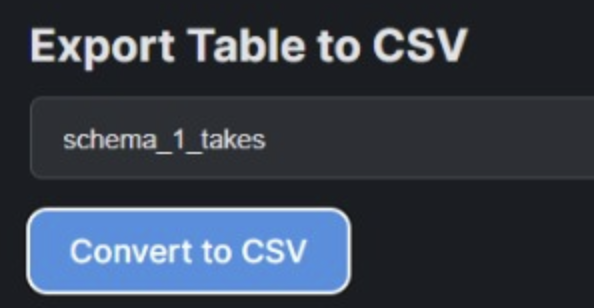
\includegraphics[width=\textwidth]{export.png}
        \caption{Export Table to CSV}
        \label{fig:export}
    \end{subfigure}
\end{figure}

\subsubsection{Exporting into different formats \ref{fig:export}}
We allow users to export the database into easy-to-read formats such as CSV, JSON, and also as a SQL dump. This allows users to easily share their databases with others, or to import them into other systems.
\subsubsection{Version Control for Databases}
We have implemented a simple version control system for the databases. Users can create a new version of the database at any time, and switch between different versions. This allows users to easily revert to a previous version of the database if needed. This feature is still a work in progress, and we plan to improve it further in the future.


\section{Implementation Details}

The key components of our code are implemented using the suggested PGLite library to ensure complete in-browser execution and compatibility with the current XData system. We have taken care to ensure that our code is modular, well-documented, easy to understand, and easy to integrate with the existing XData system. We have also tried to avoid any external dependencies to ensure that our code can run in a completely offline environment.

\subsection{Technology Stack}

We have used the following technology stack for our project:
\begin{itemize}
    \item \textbf{Frontend:} ReactJS, CSS
    \item \textbf{Build Tool:} Vite
    \item \textbf{Backend:} PGLite
\end{itemize}

\subsection{Frontend Functionality}

The frontend of our web application is built using ReactJS and CSS. We have implemented a smooth and responsive UI which allows the users to easily access all the features we have developed. Key highlights of the frontend include:

\begin{itemize}
    \item A simple and intuitive interface for users to load databases (by importing schema and data files), modify them, and run queries.
    \item Isolated tabs for each feature and a prominent navigation bar to switch between them.
    \item A Query Playground for students to test their queries and get instant feedback.
    \item Query History shown in a side panel, which allows users to easily access and retry their previous queries. 
    \item Comprehensive error messages and debugging information printed to the console.
\end{itemize}

\subsection{Backend Functionality}

The backend of our web application is built using PGLite, which allows us to run PostgreSQL queries in the browser. The database is stored in the browser's local (indexedDB) storage, which allows us to run queries without any external internet access. The key features of the backend include:

\begin{itemize}
    \item Complete support for all PostgreSQL queries, including option to EXPLAIN/ANALYZE.
    \item Support for loading multiple databases (or versions of the same database) and switching between them. Complete isolation of databases to prevent any corruption.
    \item Fully local execution of queries, with no external dependencies and a lightweight footprint.
\end{itemize}

\section{Integration with XData}

Our frontend components for managing courses, assignments, and questions were designed to interact with tables mirroring the core \texttt{XData} schema (\texttt{xdata\_course}, \texttt{xdata\_assignment}, \texttt{xdata\_qinfo}), ensuring data compatibility. We utilized the \texttt{xdata\_schemainfo} table, which allowed us to register and manage multiple dynamically loaded student database schemas within the \texttt{PGlite} environment, associating them with specific courses while maintaining the standard \texttt{XData} metadata tables within the \texttt{public} PostgreSQL schema path. This approach preserves structural alignment with \texttt{XData} while facilitating the offline, in-browser functionality central to our project goals.


\section{Programming Methodology}

Due to the nature of our project, we had to work in parallel on the frontend and backend components. We used Git/GitHub for version control so that all team members could work on the same codebase in different branches without any conflicts. 


We used LLM based tools to help us efficiently generate frontend code (mostly the styling and UI components). We observed that these tools made the development process much faster with us providing the high-level UI/UX design and the LLMs generating CSS. However, this was only possible for the frontend code (with simple components) and not for the backend code. The backend code was much more complex (especially keeping in mind the XData integration and the database schema) and required a lot of manual effort from our side to implement and debug.


\section{Future Work}
\label{sec:future-work}

We have implemented a lot of features in our project, but there is definitely room for improvement. 

Some avenues for future work include:
\begin{itemize}
    \item Adding support for more types of assignments with complex grading schemes.
    \item Allowing interaction between different databases (e.g. joining tables etc.)
    \item Adding support to change the database schema of an existing database.
    \item Integrating a better text editor for writing queries, with support for syntax highlighting and auto-completion.
    \item Improving the Syntax Constraints feature to allow more complex constraints and better error messages.
    \item Created a more robust version control system at individual transaction level with options to manually commit or rollback changes.
\end{itemize}


\section{Conclusion}

We feel that have made significant progress in our project on XData Extensions. Our team has successfully implemented several features and improvements to the existing XData system, and we have an intuitive and user-friendly web application to showcase our work. 

\medskip

Our team is very proud of the work we have done and we hope that our project will be useful for perhaps future iterations of the XData system. We are really interested to continue working on this project and fully integrate the completed features into the XData.

\subsection{Summary}
In this project, we have implemented several novel features including a Query Planner, Query Playground, Syntactic Constraints on Queries. We have created a web application from scratch using ReactJS and PGLite, which allows users to run PostgreSQL queries fully in-browser. We have also added functionality to easily import, export and modify multiple databases which work in full isolation. We have also implemented a bunch of QoL improvements such as Query History Tracker, Version Control for databases, and a convenient UI for instructors to create courses and assignments. We have also integrated some of our features with the existing XData system, and ensured that our code is modular and easy to understand. 

\subsection{Acknowledgements}

We would like to thank our instructors, Prof. S. Sudarshan and Prof. Suraj Shetiya, for their guidance and support throughout the project. Their feedback (both over email and in-person) was invaluable in helping us shape our project and implement the best set of features. We are all really grateful for their time spent with us and prompt responses to all our queries. We are also thankful to the whole XData team who built and maintain the XData system, which provided us with a great platform to build upon. We would also like to thank our peers in the course for their support and feedback during the project.

\vspace{5em}

\textit{Signing off, \\
Satyankar, Ayan, Harsh and Gourish}


\end{document}
